\documentclass{extbook}[14pt]
\usepackage{multicol, enumerate, enumitem, hyperref, color, soul, setspace, parskip, fancyhdr, amssymb, amsthm, amsmath, latexsym, units, mathtools}
\everymath{\displaystyle}
\usepackage[headsep=0.5cm,headheight=0cm, left=1 in,right= 1 in,top= 1 in,bottom= 1 in]{geometry}
\usepackage{dashrule}  % Package to use the command below to create lines between items
\newcommand{\litem}[1]{\item #1

\rule{\textwidth}{0.4pt}}
\pagestyle{fancy}
\lhead{}
\chead{Answer Key for Progress Quiz 5 Version A}
\rhead{}
\lfoot{8497-6012}
\cfoot{}
\rfoot{Summer C 2021}
\begin{document}
\textbf{This key should allow you to understand why you choose the option you did (beyond just getting a question right or wrong). \href{https://xronos.clas.ufl.edu/mac1105spring2020/courseDescriptionAndMisc/Exams/LearningFromResults}{More instructions on how to use this key can be found here}.}

\textbf{If you have a suggestion to make the keys better, \href{https://forms.gle/CZkbZmPbC9XALEE88}{please fill out the short survey here}.}

\textit{Note: This key is auto-generated and may contain issues and/or errors. The keys are reviewed after each exam to ensure grading is done accurately. If there are issues (like duplicate options), they are noted in the offline gradebook. The keys are a work-in-progress to give students as many resources to improve as possible.}

\rule{\textwidth}{0.4pt}

\begin{enumerate}\litem{
Solve the rational equation below. Then, choose the interval(s) that the solution(s) belongs to.
\[ \frac{-56}{16x -72} + 1 = \frac{-56}{16x -72} \]The solution is \( \text{all solutions are invalid or lead to complex values in the equation.} \), which is option E.\begin{enumerate}[label=\Alph*.]
\item \( x_1 \in [-5.5, -1.5] \text{ and } x_2 \in [2.5,5.5] \)

$x = -4.500 \text{ and } x = 4.500$, which corresponds to getting the correct solution and believing there should be a second solution to the equation.
\item \( x \in [-5.5,-1.5] \)

$x = -4.500$, which corresponds to not distributing the factor $16x -72$ correctly when trying to eliminate the fraction.
\item \( x \in [3.5,5.5] \)

$x = 4.500$, which corresponds to not checking if this value leads to dividing by 0 in the original equation and thus is not a valid solution.
\item \( x_1 \in [4.5, 6.5] \text{ and } x_2 \in [2.5,5.5] \)

$x = 4.500 \text{ and } x = 4.500$, which corresponds to getting the correct solution and believing there should be a second solution to the equation.
\item \( \text{All solutions lead to invalid or complex values in the equation.} \)

*$x = 4.500$ leads to dividing by 0 in the original equation and thus is not a valid solution, which is the correct option.
\end{enumerate}

\textbf{General Comment:} Distractors are different based on the number of solutions. Remember that after solving, we need to make sure our solution does not make the original equation divide by zero!
}
\litem{
Choose the equation of the function graphed below.

\begin{center}
    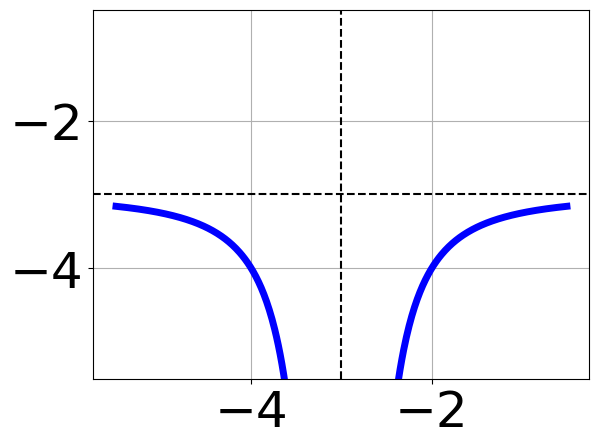
\includegraphics[width=0.5\textwidth]{../Figures/rationalGraphToEquationA.png}
\end{center}


The solution is \( f(x) = \frac{-1}{(x + 3)^2} - 3 \), which is option D.\begin{enumerate}[label=\Alph*.]
\item \( f(x) = \frac{1}{x - 3} - 3 \)

Corresponds to thinking the graph was a shifted version of $\frac{1}{x}$, using the general form $f(x) = \frac{a}{(x+h)^2}+k$, and the opposite leading coefficient.
\item \( f(x) = \frac{1}{(x - 3)^2} - 3 \)

Corresponds to using the general form $f(x) = \frac{a}{(x+h)^2}+k$ and the opposite leading coefficient.
\item \( f(x) = \frac{-1}{x + 3} - 3 \)

Corresponds to thinking the graph was a shifted version of $\frac{1}{x}$.
\item \( f(x) = \frac{-1}{(x + 3)^2} - 3 \)

This is the correct option.
\item \( \text{None of the above} \)

This corresponds to believing the vertex of the graph was not correct.
\end{enumerate}

\textbf{General Comment:} Remember that the general form of a basic rational equation is $ f(x) = \frac{a}{(x-h)^n} + k$, where $a$ is the leading coefficient (and in this case, we assume is either $1$ or $-1$), $n$ is the degree (in this case, either $1$ or $2$), and $(h, k)$ is the intersection of the asymptotes.
}
\litem{
Choose the equation of the function graphed below.

\begin{center}
    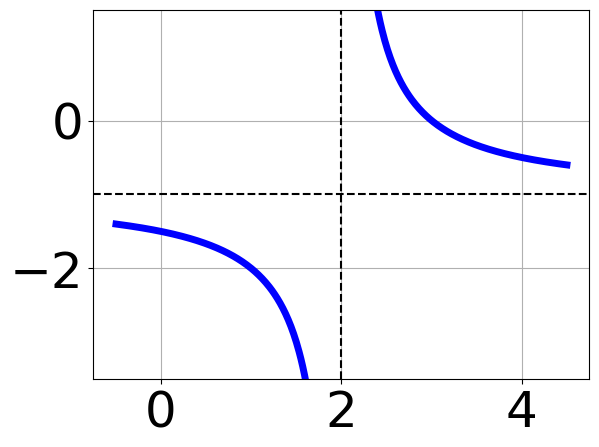
\includegraphics[width=0.5\textwidth]{../Figures/rationalGraphToEquationCopyA.png}
\end{center}


The solution is \( f(x) = \frac{1}{x - 2} - 1 \), which is option A.\begin{enumerate}[label=\Alph*.]
\item \( f(x) = \frac{1}{x - 2} - 1 \)

This is the correct option.
\item \( f(x) = \frac{1}{(x - 2)^2} - 1 \)

Corresponds to thinking the graph was a shifted version of $\frac{1}{x^2}$.
\item \( f(x) = \frac{-1}{(x + 2)^2} - 1 \)

Corresponds to thinking the graph was a shifted version of $\frac{1}{x^2}$, using the general form $f(x) = \frac{a}{x+h}+k$, and the opposite leading coefficient.
\item \( f(x) = \frac{-1}{x + 2} - 1 \)

Corresponds to using the general form $f(x) = \frac{a}{x+h}+k$ and the opposite leading coefficient.
\item \( \text{None of the above} \)

This corresponds to believing the vertex of the graph was not correct.
\end{enumerate}

\textbf{General Comment:} Remember that the general form of a basic rational equation is $ f(x) = \frac{a}{(x-h)^n} + k$, where $a$ is the leading coefficient (and in this case, we assume is either $1$ or $-1$), $n$ is the degree (in this case, either $1$ or $2$), and $(h, k)$ is the intersection of the asymptotes.
}
\litem{
Choose the graph of the equation below.
\[ f(x) = \frac{1}{(x + 3)^2} - 1 \]The solution is the graph below, which is option E.
    \begin{center}
        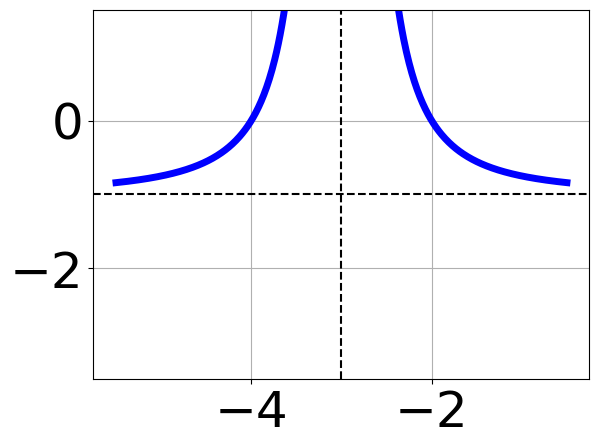
\includegraphics[width=0.3\textwidth]{../Figures/rationalEquationToGraphCopyEA.png}
    \end{center}\begin{enumerate}[label=\Alph*.]
\begin{multicols}{2}
\item 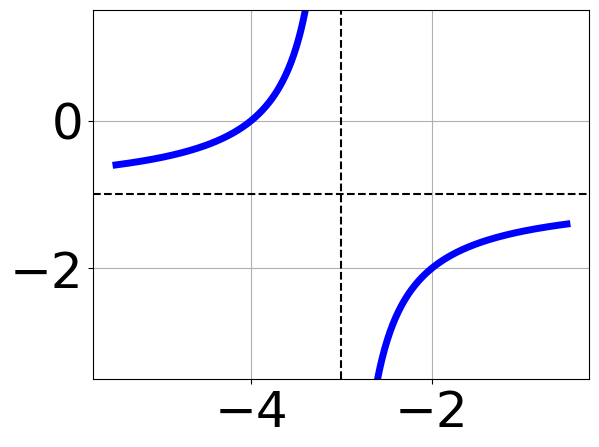
\includegraphics[width = 0.3\textwidth]{../Figures/rationalEquationToGraphCopyAA.png}
\item 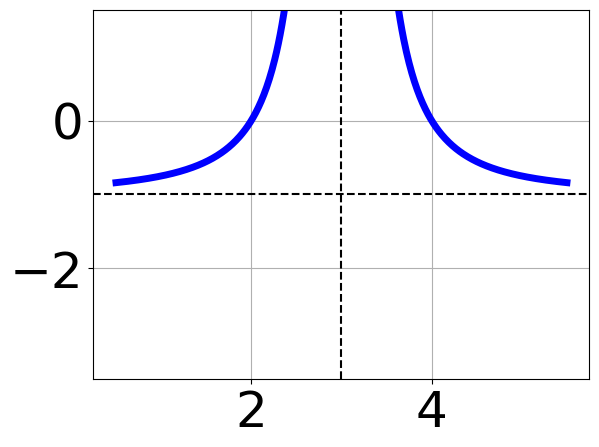
\includegraphics[width = 0.3\textwidth]{../Figures/rationalEquationToGraphCopyBA.png}
\item 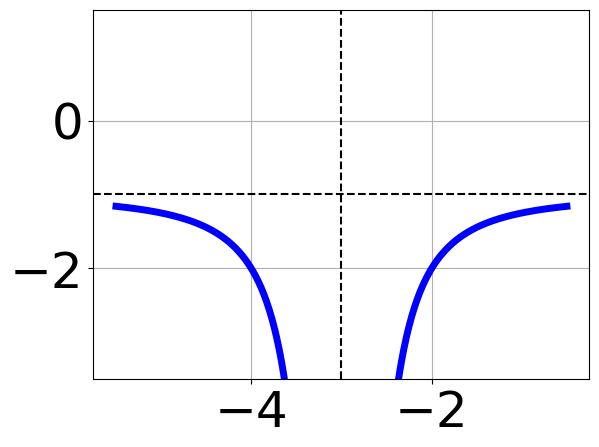
\includegraphics[width = 0.3\textwidth]{../Figures/rationalEquationToGraphCopyCA.png}
\item 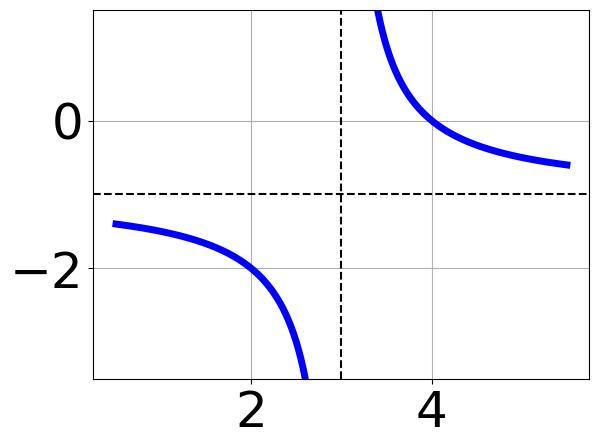
\includegraphics[width = 0.3\textwidth]{../Figures/rationalEquationToGraphCopyDA.png}
\end{multicols}\item None of the above.\end{enumerate}
\textbf{General Comment:} Remember that the general form of a basic rational equation is $ f(x) = \frac{a}{(x-h)^n} + k$, where $a$ is the leading coefficient (and in this case, we assume is either $1$ or $-1$), $n$ is the degree (in this case, either $1$ or $2$), and $(h, k)$ is the intersection of the asymptotes.
}
\litem{
Solve the rational equation below. Then, choose the interval(s) that the solution(s) belongs to.
\[ \frac{-4x}{7x + 6} + \frac{-6x^{2}}{35x^{2} -19 x -42} = \frac{-6}{5x -7} \]The solution is \( \text{There are two solutions: } x = -0.442 \text{ and } x = 3.134 \), which is option E.\begin{enumerate}[label=\Alph*.]
\item \( x \in [1.53,3.65] \)


\item \( \text{All solutions lead to invalid or complex values in the equation.} \)


\item \( x \in [0.6,1.53] \)


\item \( x_1 \in [-1.34, -0.34] \text{ and } x_2 \in [-3,2.7] \)


\item \( x_1 \in [-1.34, -0.34] \text{ and } x_2 \in [3,6.7] \)

* $x = -0.442 \text{ and } x = 3.134$, which is the correct option.
\end{enumerate}

\textbf{General Comment:} Distractors are different based on the number of solutions. Remember that after solving, we need to make sure our solution does not make the original equation divide by zero!
}
\litem{
Solve the rational equation below. Then, choose the interval(s) that the solution(s) belongs to.
\[ \frac{4x}{4x + 7} + \frac{-2x^{2}}{-8x^{2} +14 x + 49} = \frac{2}{-2x + 7} \]The solution is \( \text{All solutions are invalid or lead to complex values in the equation.} \), which is option E.\begin{enumerate}[label=\Alph*.]
\item \( x_1 \in [2.28, 3.46] \text{ and } x_2 \in [-2,3] \)

$x = 2.333 \text{ and } x = 1.000$, which corresponds to making the discriminant from the Quadratic Formula positive to avoid complex solutions.
\item \( x \in [-2.84,-0.99] \)

$x = -1.750$, which corresponds to solving $4x + 7 = 0$ and treating it as a solution to the equation.
\item \( x \in [2.68,4.19] \)

$x = 3.500$, which corresponds to solving $-2x + 7 = 0$ and treating it as a solution to the equation.
\item \( x_1 \in [-2.84, -0.99] \text{ and } x_2 \in [1.5,6.5] \)

$x = -1.750 \text{ and } x = 3.500$, which corresponds to solving $4x + 7 = 0$ and $-2x + 7 = 0$ and treating them as solutions to the equation.
\item \( \text{All solutions lead to invalid or complex values in the equation.} \)

* The equation leads to solving $-6x^{2} +20 x -14=0$, which leads to complex solutions. This is the correct option.
\end{enumerate}

\textbf{General Comment:} Distractors are different based on the number of solutions. Remember that after solving, we need to make sure our solution does not make the original equation divide by zero!
}
\litem{
Determine the domain of the function below.
\[ f(x) = \frac{6}{16x^{2} +40 x + 24} \]The solution is \( \text{All Real numbers except } x = -1.500 \text{ and } x = -1.000. \), which is option E.\begin{enumerate}[label=\Alph*.]
\item \( \text{All Real numbers except } x = a, \text{ where } a \in [-1.67, -1.4] \)

All Real numbers except $x = -1.500$, which corresponds to removing only 1 value from the denominator.
\item \( \text{All Real numbers except } x = a \text{ and } x = b, \text{ where } a \in [-24.11, -23.87] \text{ and } b \in [-16.78, -15.56] \)

All Real numbers except $x = -24.000$ and $x = -16.000$, which corresponds to not factoring the denominator correctly.
\item \( \text{All Real numbers except } x = a, \text{ where } a \in [-24.11, -23.87] \)

All Real numbers except $x = -24.000$, which corresponds to removing a distractor value from the denominator.
\item \( \text{All Real numbers.} \)

This corresponds to thinking the denominator has complex roots or that rational functions have a domain of all Real numbers.
\item \( \text{All Real numbers except } x = a \text{ and } x = b, \text{ where } a \in [-1.67, -1.4] \text{ and } b \in [-1.32, -0.74] \)

All Real numbers except $x = -1.500$ and $x = -1.000$, which is the correct option.
\end{enumerate}

\textbf{General Comment:} Recall that dividing by zero is not a real number. Therefore the domain is all real numbers \textbf{except} those that make the denominator 0.
}
\litem{
Determine the domain of the function below.
\[ f(x) = \frac{6}{16x^{2} +8 x -15} \]The solution is \( \text{All Real numbers except } x = -1.250 \text{ and } x = 0.750. \), which is option E.\begin{enumerate}[label=\Alph*.]
\item \( \text{All Real numbers except } x = a, \text{ where } a \in [-23, -19] \)

All Real numbers except $x = -20.000$, which corresponds to removing a distractor value from the denominator.
\item \( \text{All Real numbers.} \)

This corresponds to thinking the denominator has complex roots or that rational functions have a domain of all Real numbers.
\item \( \text{All Real numbers except } x = a, \text{ where } a \in [-4.25, -0.25] \)

All Real numbers except $x = -1.250$, which corresponds to removing only 1 value from the denominator.
\item \( \text{All Real numbers except } x = a \text{ and } x = b, \text{ where } a \in [-23, -19] \text{ and } b \in [12, 13] \)

All Real numbers except $x = -20.000$ and $x = 12.000$, which corresponds to not factoring the denominator correctly.
\item \( \text{All Real numbers except } x = a \text{ and } x = b, \text{ where } a \in [-4.25, -0.25] \text{ and } b \in [0.75, 2.75] \)

All Real numbers except $x = -1.250$ and $x = 0.750$, which is the correct option.
\end{enumerate}

\textbf{General Comment:} Recall that dividing by zero is not a real number. Therefore the domain is all real numbers \textbf{except} those that make the denominator 0.
}
\litem{
Choose the graph of the equation below.
\[ f(x) = \frac{-1}{x - 1} + 2 \]The solution is the graph below, which is option E.
    \begin{center}
        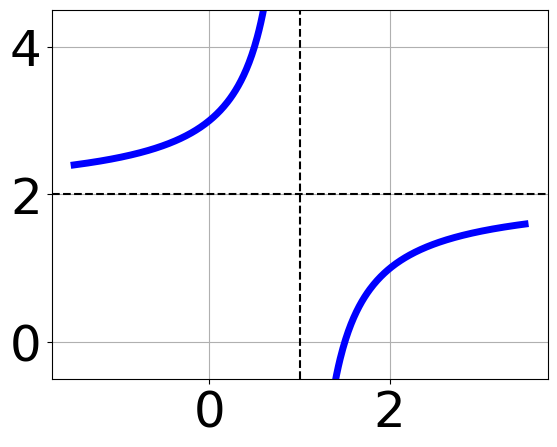
\includegraphics[width=0.3\textwidth]{../Figures/rationalEquationToGraphEA.png}
    \end{center}\begin{enumerate}[label=\Alph*.]
\begin{multicols}{2}
\item 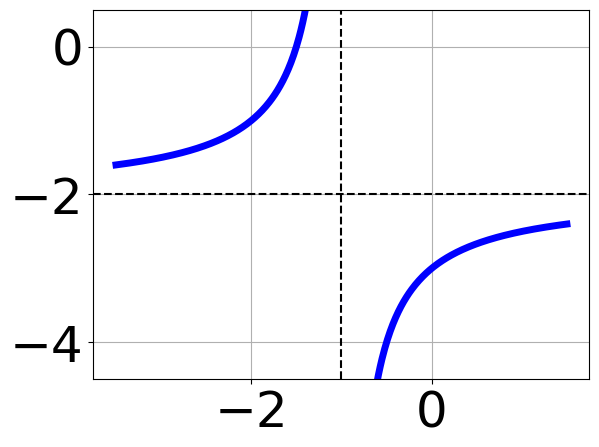
\includegraphics[width = 0.3\textwidth]{../Figures/rationalEquationToGraphAA.png}
\item 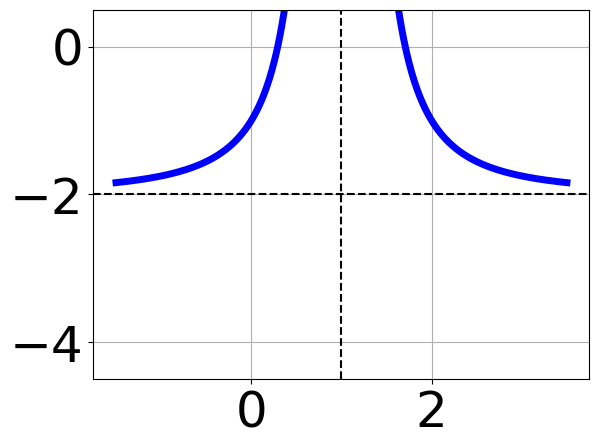
\includegraphics[width = 0.3\textwidth]{../Figures/rationalEquationToGraphBA.png}
\item 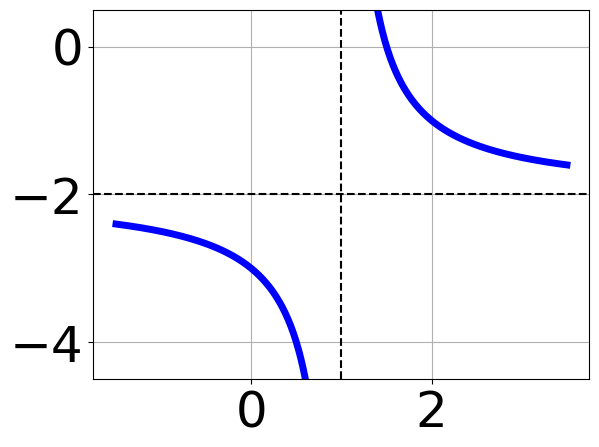
\includegraphics[width = 0.3\textwidth]{../Figures/rationalEquationToGraphCA.png}
\item 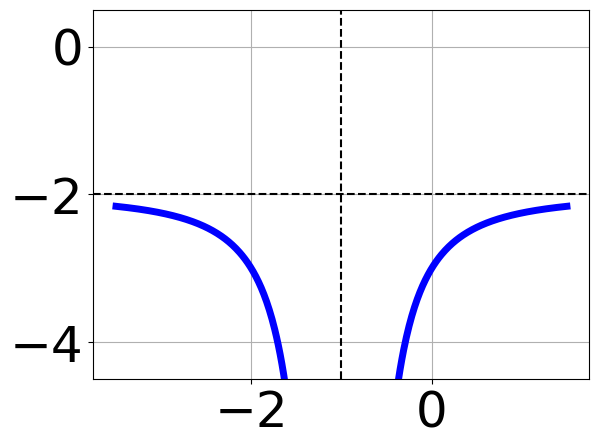
\includegraphics[width = 0.3\textwidth]{../Figures/rationalEquationToGraphDA.png}
\end{multicols}\item None of the above.\end{enumerate}
\textbf{General Comment:} Remember that the general form of a basic rational equation is $ f(x) = \frac{a}{(x-h)^n} + k$, where $a$ is the leading coefficient (and in this case, we assume is either $1$ or $-1$), $n$ is the degree (in this case, either $1$ or $2$), and $(h, k)$ is the intersection of the asymptotes.
}
\litem{
Solve the rational equation below. Then, choose the interval(s) that the solution(s) belongs to.
\[ \frac{108}{72x -36} + 1 = \frac{108}{72x -36} \]The solution is \( \text{all solutions are invalid or lead to complex values in the equation.} \), which is option E.\begin{enumerate}[label=\Alph*.]
\item \( x \in [-0.9,-0.2] \)

$x = -0.500$, which corresponds to not distributing the factor $72x -36$ correctly when trying to eliminate the fraction.
\item \( x_1 \in [-0.9, -0.2] \text{ and } x_2 \in [-0.5,2.5] \)

$x = -0.500 \text{ and } x = 0.500$, which corresponds to getting the correct solution and believing there should be a second solution to the equation.
\item \( x \in [0.5,2.5] \)

$x = 0.500$, which corresponds to not checking if this value leads to dividing by 0 in the original equation and thus is not a valid solution.
\item \( x_1 \in [0.2, 1.1] \text{ and } x_2 \in [-0.5,2.5] \)

$x = 0.500 \text{ and } x = 0.500$, which corresponds to getting the correct solution and believing there should be a second solution to the equation.
\item \( \text{All solutions lead to invalid or complex values in the equation.} \)

*$x = 0.500$ leads to dividing by 0 in the original equation and thus is not a valid solution, which is the correct option.
\end{enumerate}

\textbf{General Comment:} Distractors are different based on the number of solutions. Remember that after solving, we need to make sure our solution does not make the original equation divide by zero!
}
\end{enumerate}

\end{document}